\textbf{Входные параметры:}
 
 x --- входная переменная.

\textbf{Возвращаемое значение:}

 Значение функции в точке.
 
\textbf{Формула:}
\begin{equation*}
F\left(x \right)=\dfrac{1}{\sqrt{2\pi}}e^{-\dfrac{x^2}{2}}.
\end{equation*}

 \begin{figure} [h] 
   \center
   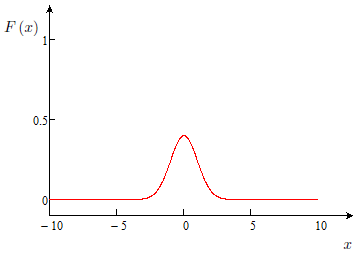
\includegraphics {HML_DensityOfDistributionOfNormalizedCenteredNormalDistribution_Graph.png}
   \caption{График функции} 
   \label{img:HML_DensityOfDistributionOfNormalizedCenteredNormalDistribution_Graph}  
 \end{figure}
 
